\section{Problem Description}\label{sec:prob_descr}

\subsection{Hardware setup}
The helicopter is fixed to a base and has an extended arm with motors attached at one end,
and a balance weight at the other. We parametrize the helicopter state by three rotations:
\begin{itemize}
    \item Travel ($\lambda$): At the base about the vertical axis
    \item Elevation ($e$): At the arm joint about a horizontal axis
    \item Pitch ($p$): At the head joint about the arm axis
\end{itemize}
These angles are measured by the encoders at each rotational joint. We can affect the motion by adjusting the voltage input to the DC motors. Propellers are attached to the motors, and the thrust generated is assumed to be proportional to the voltage applied, with identical motor constant for both motors. Figure (\ref{fig:hardware}) shows the helicopter and the relevant angles. Table (\ref{tab:parameters}) shows the parameters for the helicopter used in the report.

\begin{figure}[htb]
	\centering
	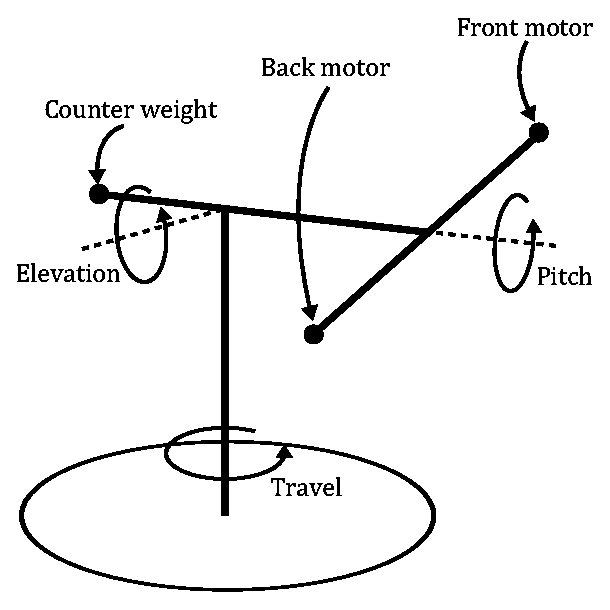
\includegraphics[width = 0.6\textwidth]{figures/hardware_setup.eps}
	\caption{The helicopter hardware setup}
	\label{fig:hardware}
\end{figure}

\subsection{Software setup}
We use Simulink and Matlab to implement the control program, and interface with the helicopter through QuaRC and Realtime Workshop. See [\cite{LabExercise}] for more information.

\subsection{Model discussion}
In order to compute an optimal control input, we need some measure of optimality.
To this extent, we use a discrete-time state-space model, that describes the motion
of our helicopter given an input sequence. The first step is to derive the equations
of motions in continuous-time. We do this by considering torque balances about each
rotation axis, and applying Newton's law. A full derivation is not interesting, so
we refer to the exercise text [\cite{LabExercise}] and list the resulting set of
differential equations below.
\begin{subequations}
\label{eq:model_al}
\begin{align}
    \ddot{e} + K_{3} K_{ed} \dot{e} + K_{3} K_{ep} e &= K_{3} K_{ep} e_{c} \label{eq:model_se_al_elev} \\
    \ddot{p} + K_{1} K_{pd} \dot{p} + K_{1} K_{pp} p &= K_{1} K_{pp} p_{c} \label{eq:model_se_al_pitch} \\
    \dot{\lambda} &= r \label{eq:model_se_al_lambda} \\
    \dot{r} &= -K_{2} p \label{eq:model_se_al_r}
\end{align}
\end{subequations}

The associated nomenclature is listed in table (\ref{tab:variables}). This model deserves some discussion. First, a complete model would have (non-linear) trigonometric terms. But such a model is impractical for use in dynamic optimization schemes. Instead, we linearize the model by assuming that the pitch and elevation angles are both close to zero.

The resulting model has the advantage of being compatible with highly efficient techniques that have been developed specifically for linear optimization problems. It is however a very simple model, and omits any interaction between elevation and pitch angle/travel. While there will always be modelling errors due to process noise, or inaccurate measurements/parameters, this simplification will affect the computed optimal control. We can dampen the effect from the error by keeping the system close to the linearization point, for instance by constraining the angles to be within a margin around equilibrium.

Second, the model incorporates a PID controller for the elevation, which is assumed to counteract the constant torque due to gravity, as well as a PD controller for the pitch. The result of this is that our goal in the optimization problem is to compute the setpoints, $e_c$ and $p_c$. Computing the appropriate voltages is left to the internal controllers.

\newpage
\begin{table}[ht]
    \centering
    \caption{Parameters and values}
    \begin{tabular}{llll}
        \hline
        Symbol & Parameter & Value & Unit \\
        \hline
        $l_a$ & Distance from elevation axis to helicopter body & $0.63$ & \meter \\
        $l_h$ & Distance from pitch axis to motor & $0.18$ & \meter \\
        $K_f$ & Force constant motor & $0.20$ & \newton\per\volt \\
        $J_e$ & Moment of inertia for elevation & $1.11$ & \kilogram\usk\square\meter \\
        $J_t$ & Moment of inertia for travel & $1.11$ & \kilogram\usk\square\meter \\
        $J_p$ & Moment of inertia for pitch & $0.045$ & \kilogram\usk\square\meter \\
        $m_h$ & Mass of helicopter & $1.42$ & \kilogram \\
        $m_w$ & Balance weight & $1.80$ & \kilogram \\
        $m_g$ & Effective mass of the helicopter & $0.025$ & \kilogram \\
        $K_p$ & Force to lift the helicopter from the ground & $0.25$ & \newton \\
        \hline
    \end{tabular}
    \label{tab:parameters}
\end{table}

\begin{table}[ht]
    \centering
    \caption{Variables}
    \begin{tabular}{ll}
    \hline
    Symbol & Variable \\
    \hline
    $p$                    & Pitch \\
    $p_c$                  & Setpoint for pitch \\
    $\lambda$              & Travel \\
    $r$                    & Speed of travel \\
    $r_c$                  & Setpoint for speed of travel \\
    $e$                    & Elevation \\
    $e_c$                  & Setpoint for elevation \\
    $V_f$                  & Voltage, motor in front \\
    $V_b$                  & Voltage, motor in back \\
    $V_d$                  & Voltage difference, $V_f - V_b$ \\
    $V_s$                  & Voltage sum, $V_f + V_b$ \\
    $K_{pp},K_{pd},K_{ep},K_{ei}, K_{ed}$ & Controller gains \\
    $T_g$                  & Moment needed to keep the helicopter flying \\
    $\lambda^*$        & Optimal travel trajectory \\
    $p_c^*$               & Optimal pitch setpoint \\
    $e_c^*$               & Optimal elevation setpoint \\
    \hline
    \end{tabular}
    \label{tab:variables}
\end{table}
